% Ubah judul dan label berikut sesuai dengan yang diinginkan.
\section{Methodology}
\label{sec:arsitektur}

\subsection{You Only Look Once (YOLO) Model}
\label{subsec:yolo_base}

\par \emph{You Only Look Once} atau YOLO adalah algoritma \emph{multi object detection} yang sangat cepat yang dicetuskan oleh Redmot et al pada tahun 2015 lewat buku mereka \emph{You Only Look Once: Unified, Real-Time Object Detection} \cite{redmon2016you}. \emph{Convolutional Neural Network} menjadi basis dari sistem deteksi YOLO ini. YOLO melakukan deteksi objek dengan menganggap nya sebagai pemrasalahan regresi tunggal yang diambil langsung dari \emph{pixel - pixel} yang ada di gambar menjadi \emph{bounding box} penanda dari koordinat - koordinat dan probabilitas dari klasifikasinya. Dengan begitu hanya perlu dilakukan satu kali pengecekan pada gambar untuk melakukan deteksi atau indentifikasi. \cite{redmon2016you} YOLO menggabungkan beberapa komponen dari teksi objek menjadi satu neural network yang dimana menggunakan fitu-fitur dari seluruh bagian gambar untuk memprediksi tiap \emph{bounding box} sekaligus melakukan prediksi untuk semua \emph{bounding box} di semua tipe klasifikasi yang ada. Desain dari YOLO ini memungkinkan untuk melakukan \emph{end to end training} dan kecepatan deteksi \emph{real time}.

\par Sistem dari YOLO sendiri membagi input gambar menjadi grid S x S. Grid disini perannya untuk nanti yaitu jika grid tertentu menjadi pusat dari objek maka grid tersebut yang nantinya berguna untuk deteksi objek tadi.

\par Setiap grid memprediksi tiap bound box dan nilai kemungkinan klasifikasi atau \emph{confidence score} dari \emph{bounding box} tersebut. Nilai tersebut mewakili seberapa "yakin" model akan objek yang terdeteksi di bounding box dan seberapa akurat prediksinya. 

\par Terdapat lima nilai prediksi yang ada pada tiap bounding box yaitu : x, y, w, h, dan \emph{confidence}. X dan Y mewakili pusat dari bounding box. W dan H mewakili \emph{Weight} dan \emph{Height} diprediksi relatif dari seluruh gambar. Lalu \emph{confidence score} sendiri mewakili IOU antara \emph{predicted box} dan \emph{ground truth box} \cite{redmon2016you}.

\subsubsection{YOLOv5}
\label{subsecsec:yolov5}

% \par YOLOv5 is an updated version of YOLO which was created in 2020 by Glenn Jocher \cite{glenn_jocher_yolov5}. Based on the Github repository for YOLOv5 by Glenn Jocher, the network structure of YOLOv5 is divided into 3 main parts, namely Backbone, Neck, and Head modules. As can be seen in Figure \ref{fig:yolov5network}. 

% \par The network structure of YOLOv5 starts from the Backbone module where the input image is passed first to extract features from the image whose structure is based on CSP-Darknet53. But before going through the Backbone, the input image are being pass through the Focus structure. Inside the backbone, the input go through several  Bottleneck CSP Networks (Cross Stage Partial Networks) and then  and Spatial Pyramid Pooling (SPP). The main purpose of the Spatial Pyramid Pooling block is to generate output with the same size regardless of the size of the input frame. The result of feature extraction from Backbone is then used to generate \emph{feature pyramid} in the Neck module which is a structure based on PANet (Path Aggregation Network). Finally, in the Head Module, the information needed to draw bounding box and to tell what class is being detected is generated here which includes some information, namely: class, coordinates, and confidence score.

\par YOLOv5 adalah versi terbaru dari YOLO yang dibuat pada tahun 2020 oleh Glenn Jocher \cite{glenn_jocher_yolov5}. Berdasarkan repositori Github untuk YOLOv5 oleh Glenn Jocher, struktur jaringan YOLOv5 dibagi menjadi 3 bagian utama, yaitu modul Backbone, Neck, dan Head. Seperti dapat dilihat pada Gambar \ref{fig:yolov5network}.

\par Struktur jaringan YOLOv5 dimulai dari modul Backbone di mana gambar input dilewatkan terlebih dahulu untuk mengekstrak fitur dari gambar yang strukturnya didasarkan pada CSP-Darknet53. Namun sebelum melalui Backbone, gambar input melewati struktur Focus. Di dalam backbone, input melewati beberapa Jaringan CSP Bottleneck (Cross Stage Partial Networks) dan kemudian Spatial Pyramid Pooling (SPP). Tujuan utama dari blok Spatial Pyramid Pooling adalah untuk menghasilkan output dengan ukuran yang sama terlepas dari ukuran frame input. Hasil ekstraksi fitur dari Backbone kemudian digunakan untuk menghasilkan \emph{feature pyramid} pada modul Neck yang merupakan struktur berbasis PANet (Path Aggregation Network). Terakhir, di Head Module, informasi yang diperlukan untuk menggambar kotak pembatas dan untuk memberi tahu kelas apa yang terdeteksi dihasilkan di sini yang mencakup beberapa informasi, yaitu: kelas, koordinat, dan skor kepercayaan.

\begin{figure*} [ht]
  \centering
  % Ubah sesuai dengan nama file gambar dan ukuran yang akan digunakan.
  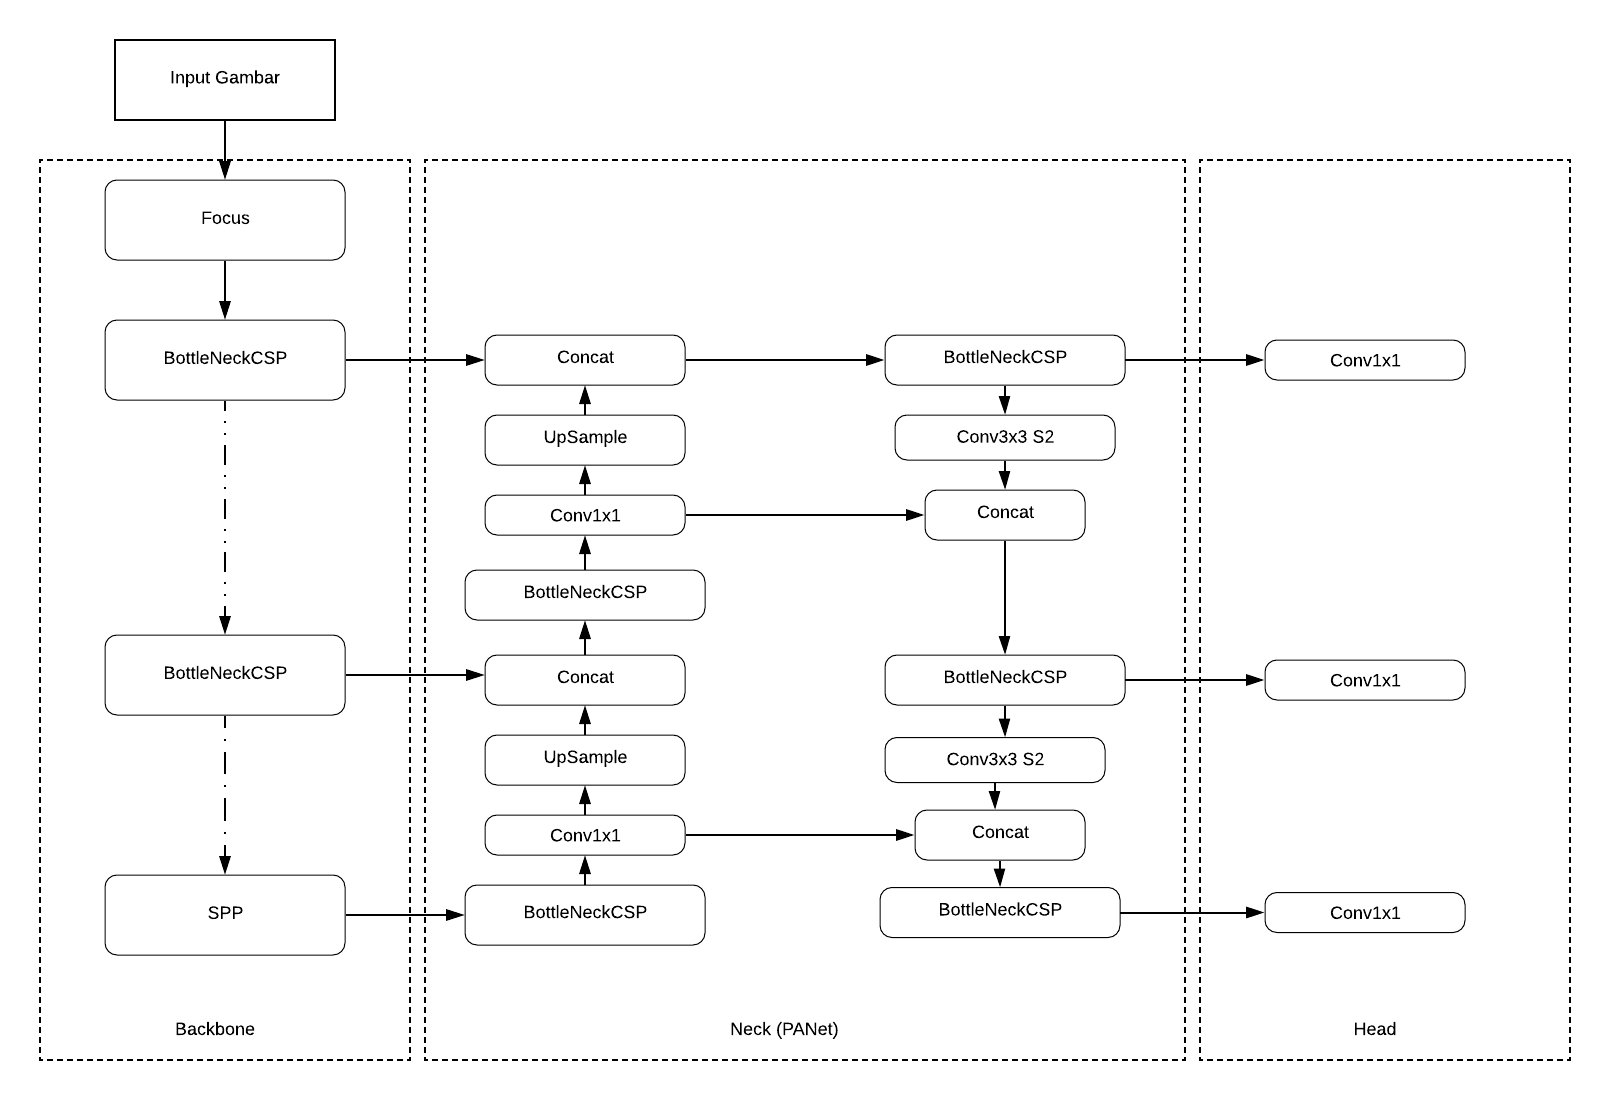
\includegraphics[width=0.9\textwidth]{gambar/yolov5 structure.png}

  % Ubah sesuai dengan keterangan gambar yang diinginkan.
  \caption{Arsitektur YOLOv5}
  \label{fig:yolov5network}
\end{figure*}

\subsection{Alat dan Bahan}
\label{subsec:toolsandequipment}

\par Dalam mengerjakan judul penelitian ini, ada beberapa alat dan perlengkapan yang digunakan untuk menyelesaikan penelitian ini, mulai dari alat yang berupa perangkat lunak dan perangkat keras. Berikut ini adalah penjelasan dari alat-alat yang digunakan.

\begin{enumerate}[nolistsep]
  \item Desktop Computer
  \item Google Colab
  \item Jetson Nano
  \item Webcam Nemesis NYK A-90 Everest
\end{enumerate}

\begin{table} [ht]
  \caption{Spesifikasi Desktop Computer}
  \label{tab:desktopspec}
  \centering
  \begin{tabular}{|c|c|}
    \hline
    % \rowcolor[HTML]{C0C0C0}
    \textbf{Type} & \textbf{Detail}  \\
    \hline
    \textit{Processor} & AMD Ryzen 5 2600 \\ 
    Memory             & 16 GB  \\
    Storage            & HDD 1TB SSD 1,256 TB\\
    Graphic Card       & NVIDIA GeForce GTX 1060 6GB \\
    Operating System   & Windows 10     \\
    CUDA               & CUDA version 11.2    \\              
    \hline
  \end{tabular}
\end{table}

\begin{table} [ht]
  \caption{Spesifikasi Jetson Nano}
  \label{tab:jetsonspec}
  \centering
  \begin{tabular}{|c|c|}
    \hline
    \textbf{Type} & \textbf{Detail}  \\
    \hline
    \textit{Processor} & Quad-core ARM Cortex-A57 MPCore processor \\ 
    Memory             & 4 GB 64-bit LPDDR4, 1600MHz 25.6 GB/s  \\
    Storage            & SDCARD 512 GB\\
    Graphic Card       & NVIDIA Maxwell architecture \\
                      & with 128 NVIDIA CUDA® cores \\
    Operating System   & Ubuntu     \\
    CUDA               & CUDA version 10.2.300    \\              
    \hline
  \end{tabular}
\end{table}

\begin{table} [ht]
  \caption{Spesifikasi Nemesis NYK A-90 Everest Webcam}
  \label{tab:nyka90_webcam_spec}
  \centering
  \begin{tabular}{|c|c|}
    \hline
    % \rowcolor[HTML]{C0C0C0}
    \textbf{Type} & \textbf{Detail}  \\
    \hline
    Resolution         & 1920x1080 \\ 
    Max FPS            & 30 FPS  \\
    Other Detail       & Full 360 Degree Rotation \\
                        & Auto Focus \\
                        & Auto Exposure White Balance    \\
                      & Full HD Glass Lens    \\              
    \hline
  \end{tabular}
\end{table}

\subsection{Workflow}
\label{subsec:workflow}

\par Tata cara pengerjaan judul Tugas Akhir ini dibagi menjadi beberapa tahapan berdasarkan metodologi yang telah disusun seperti terlihat pada Gambar~\ref{fig:hedec_method}, yaitu:

\begin{enumerate}[nolistsep]  
  \item Akuisisi Dataset
  \item Dataset Labeling 
  \item Dataset Preprocessing  
  \item Dataset Training dengan Yolov5  
  \item Pengembangan Sistem Deteksi Helm Keselamatan Kerja
  \item Implementasi Sistem Deteksi Helm Keselamatan Kerja 
  \item Evaluasi Hasil Implementasi
\end{enumerate}

\begin{figure*} [ht]
  \centering
  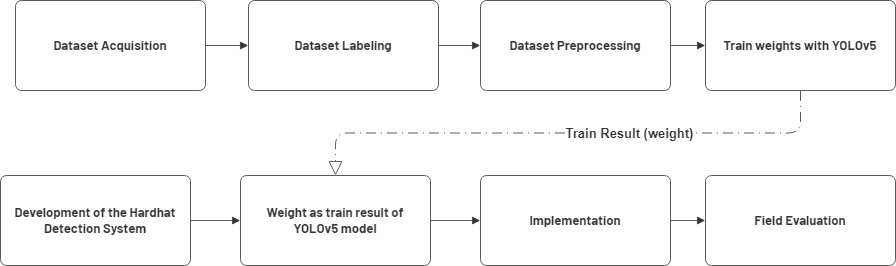
\includegraphics[width=0.9\textwidth]{gambar/utilities/methodologi_hardhat.png}

  \caption{Metodologi Deteksi Helm Keselamatan Kerja}
  \label{fig:hedec_method}
\end{figure*}

\subsection{Akuisisi Dataset}
\label{subsec:DatasetAcquisition}

\par Dataset yang digunakan untuk training menggunakan Yolov5 berupa dataset berisi gambar - gambar yang mengandung personel lapangan proyek yang mengenakan helm dan yang tidak mengenakan helm. Untuk penelitian ini, dataset yang digunakan berasal dari dua sumber yaitu :

\begin{enumerate}
  \item Safety Helmet Detection oleh andrewmvd
  \par Dataset ini berisi 5000 gambar pekerja konstruksi yang meliputi orang yang menggunakan helm dan yang tidak menggunakan helm keselamatan kerja. Masin - masing gambar sudah diberi label ”helmet” dan ”head”. Format anotasi label nya berupa fromat PASCAL VOC yang disimpan dalam file .xml. Beberap sampel gambar dari dataset ini dapat dilihat pada Gambar~\ref{fig:datasethelmetdetectionpreview}

  \begin{figure}[ht]
    \centering
    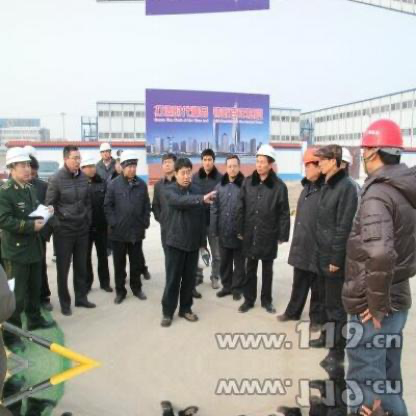
\includegraphics[width=0.24\textwidth]{gambar/sample_kaggle1/hard_hat_workers0.png}
    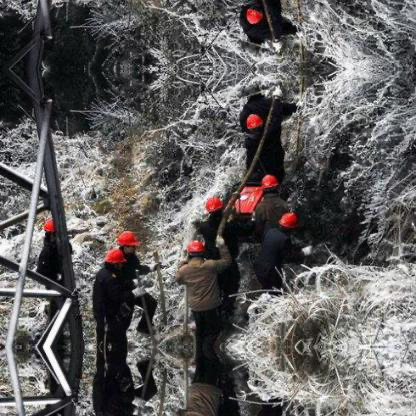
\includegraphics[width=0.24\textwidth]{gambar/sample_kaggle1/hard_hat_workers1.png}
    \caption{Dataset \emph{Safety Helmet Detection} oleh andrewmvd}
    \label{fig:datasethelmetdetectionpreview}  
  \end{figure}

  \item SampleERASTY2020 dataset oleh Alif Aditya Wicaksono
  \par Dataset ini berisi 8.867 gambar yang kandungannya serupa dengan dataset Safety Helmet Detection oleh andrewmvd sebelumnya. Dataset ini juga sudah lengkap dengan annotasi nya tetapi membutuhkan beberapa perubahan untuk disesuaikan dengan  metode trainingnya. Selain itu, 8.867 gambar tersebut juga sudah termasuk hasil augmentasi seperti flip, rotation, blur, dan noise. Sampel gambar dari dataset ini dapat dilihat pada Gambar~\ref{fig:dataseterastypreview}

  \begin{figure}[ht]
    \centering
    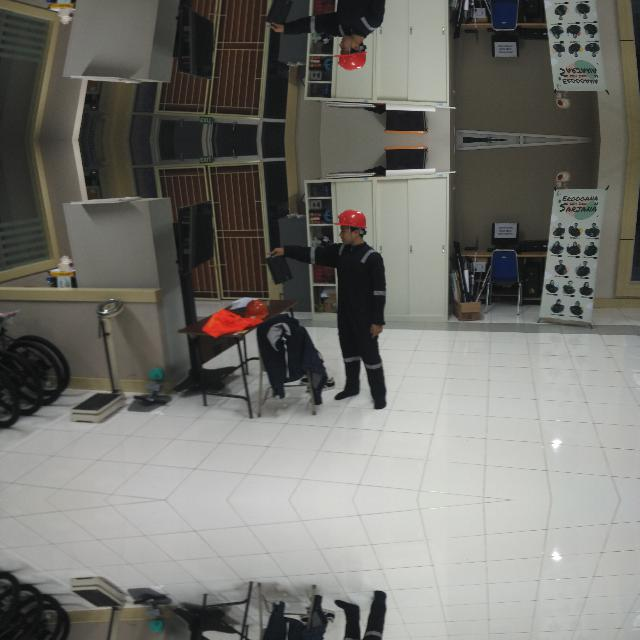
\includegraphics[width=0.24\textwidth]{gambar/sample_erasty/APB-Hat-6-_jpg.rf.79aa17f23c1834efa681edc7aca5cd5f.jpg}
    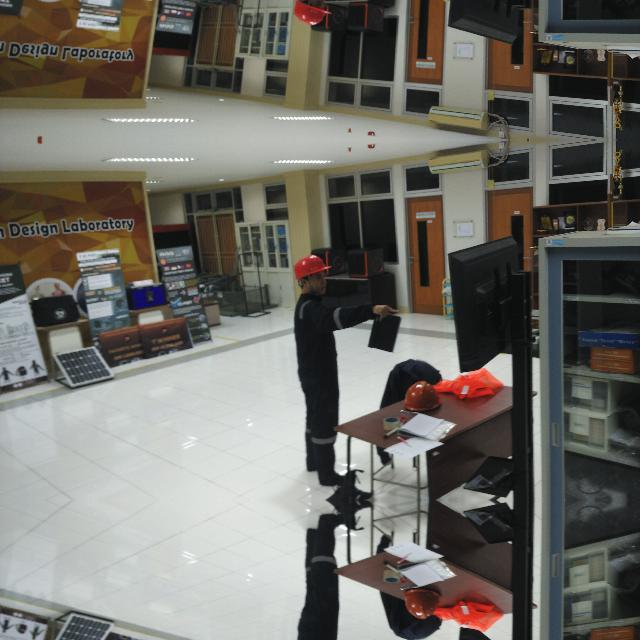
\includegraphics[width=0.24\textwidth]{gambar/sample_erasty/APB-Hat-7-_jpg.rf.4e9ff94579f598546de38a9b5c88a05d.jpg}
    \caption{Dataset SampleERASTY2020 oleh Alif Aditya Wicaksono}
    \label{fig:dataseterastypreview}  
  \end{figure}

\end{enumerate}

\subsection{Dataset Labeling}
\label{subsec:dataset_labeling}

\par Kumpulan dataset yang telah dikumpulkan sebelumnya di Subbagian~\ref{subsec:DatasetAcquisition} harus memiliki anotasi sebelum digunakan sebagai dataset untuk keperluan \emph{training}. Ada dua kelas yang digunakan untuk sistem ini:

\begin{enumerate}[nolistsep]
  \item "with\textunderscore helmet" yang meliputi kepala dan helm keselamatan kerja
  \item “no\textunderscore helmet” yang meliputi kepala tanpa helm keselamatan kerja
\end{enumerate}

Pada dataset yang sudah didapatkan sudah memiliki pelabelan atau anotasi nya masing - masing, tetapi khusus untuk dataset SampleERASTY2020 terdapat ketidak sesuaian untuk label Hard-hat dimana hanya meliputi helm keselamatan kerja tanpa kepala penggunananya. Maka dari itu  dilakukan pelabelan ulang untuk dataset SampleERASTY2020 dimana hanya menggunakan file gambar yang masih belum hasil augmentasi yang berjumlah 338 gambar. Proses pelabelan gambar dilakukan di platform Roboflow seperti yang terlihat di Gambar~\ref{fig:gambarbesertalabel}

\begin{figure}[ht]
  \centering
  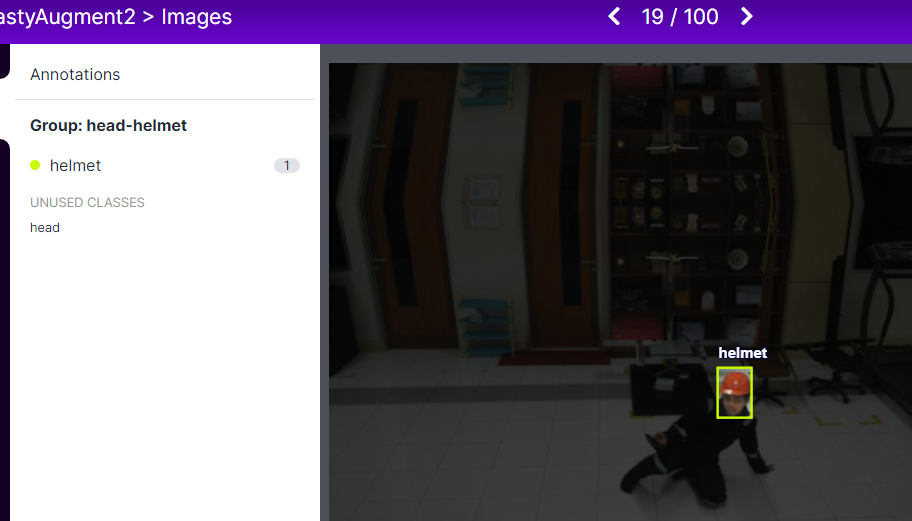
\includegraphics[width=0.4\textwidth]{gambar/utilities/labeldiroboflow.png}
  \caption{Image Labeling di Roboflow}
  \label{fig:gambarbesertalabel}  
\end{figure}

\subsection{Dataset Preprocessing}
\label{subsec:dataset_preprocessing}

\par Ada beberapa proses yang dilakukan untuk dataset yang sudah dikumpulkan agar bisa digunakan untuk proses training dengan benar. Proses tersebut meliputi pengaturan ulang ukuran gambar atau \emph{resizing}, penamaan ulang nama kelas, dan augmentasi. Untuk penelitian ini, proses - proses tersebut dilakukan pada platform Roboflow.

\subsubsection{Mengatur Ulang Ukuran Gambar}
\label{subsec:imageresize}
\par YOLOv5 yang digunakan untuk men-train dataset menerima gambar dalam ukuran 640x640 dengan warna RGB sehingga dataset yang ada akan diresize dalam ukuran tersebut. Source code YOLOv5 dari repository github sebenarnya sudah menyediakan fitur resize sebelum di train tetapi dari penulis melakukan resize menggunakan roboflow.  

\subsubsection{Membersihkan Dataset}
\label{subsec:datasetcleanup}
\par Terdapat beberapa gambar yang tidak diperlukan dari dataset yang didapatkan seperti gambar yang hanya memiliki gambar rompi proyek yang dimana tidak digunakan untuk keperluan training. Untuk beberapa gambar tersebut akan tidak diikutkan dalam export dataset dari roboflow.

\subsubsection{Penamaan Ulang Nama Kelas Pada Dataset SampleERASTY2020}
\label{subsec:classrename}
\par Penamaan kelas  label yang ada dari dataset yang sudah ada akan disesuaikan untuk keperluan penggunaan dan pemahaman yang lebih mudah. Dataset SampleERASTY2020 yang sudah dilabel ulang tidak perlu melewati proses ini tetapi untuk dataset Safety Helmet Detection perlu dilakukan penamaan ulang dimana untuk class “helmet” menjadi “with\textunderscore helmet” dan “head” menjadi “no\textunderscore helmet” seperti yang ditunjukan pada Gambar \ref{fig:prepro_classrename}. 

\begin{figure}[ht]
  \centering
  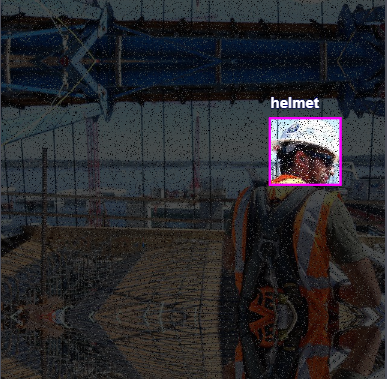
\includegraphics[width=0.24\textwidth]{gambar/utilities/reclass_old.png}
  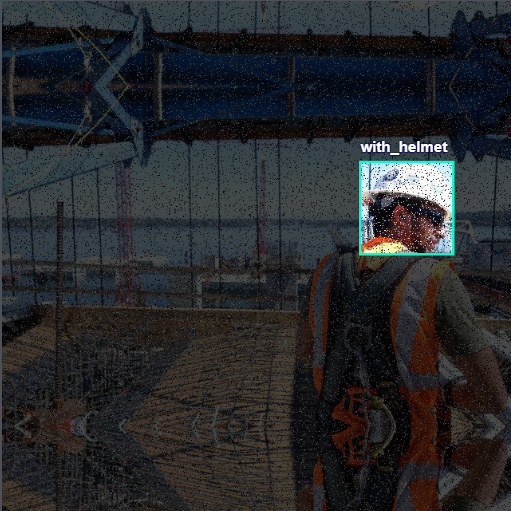
\includegraphics[width=0.24\textwidth]{gambar/utilities/reclass_new.png}
  \caption{Class Rename in Roboflow}
  \label{fig:prepro_classrename}  
\end{figure}

\subsubsection{Augmentasi Dataset}
\label{subsec:augmentation}
\par Augmentasi tambahan juga dilakukan pada dataset untuk menambah variasi gambar pada dataset dimana untuk bentuk augmentasi yang digunakan yaitu \emph{noise} dan \emph{horizontal flip}. Proses augmentasi dilakukan di platform \emph{Roboflow} yang juga menyediakan fitur augmentasi. Dataset SampleERASTY2020 yang sudah dilabel ulang dan diaugmentasi tambahan lali digabungkan dengan dataset yang sudah didapatkan sebelumnya yang berjumlah 5000 gambar. 

\begin{figure}[ht]
  \centering
  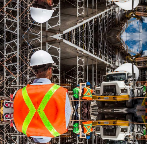
\includegraphics[width=0.24\textwidth]{gambar/utilities/aug_flip.png}
  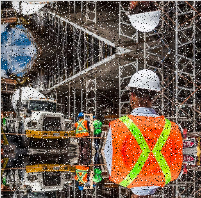
\includegraphics[width=0.24\textwidth]{gambar/utilities/aug_noise.png}
  \caption{\emph{Flip} and \emph{Noise} Augmentation}
  \label{fig:prepro_augmentasi}  
\end{figure}

\subsubsection{Pembagian Dataset}
\label{subsec:datasetsubset}
\par Sebelum digunakan untuk men-\emph{traing} \emph{weight}, dataset yang sebelumnya sudah digabungkan perlu ditentukan pembagiannya untuk set \emph{train - test - val}-nya. Pembagian untuk dataset yang digunakan untuk training yaitu 70\% train (4202) , 20\% test (1.200 gambar), dan 10\% validation (600 gambar). Untuk \emph{training} menggunakan YOLOv5 yang berbasis \emph{PyTorch}, \emph{Roboflow} menyediakan fitur \emph{export} dataset ke format yang ditentukan dimana disini anotasinya disimpan dalam bentuk \emph{.txt} dan diatur lewat file \emph{.yaml} Pembagian dataset ini dilakukan melalui fitur \emph{Generate Dataset Version} pada platform \emph{Roboflow}. Dataset yang didapat dari proses penggabungan dataset yang disebutkan pada Subbab~\ref{subsec:DatasetAcquisition} dan setelah melalui \emph{pre-processing} selanjutnya akan disebut sebagai Dataset Helm Keselamatan Kerja untuk mempersingkat.

\subsection{Training}
\label{subsec:dataset_training}

\par Dataset - dataset yang sudah di pre-process sebelumnya di roboflow dan sudah memiliki anotasi yang susai lalu digunakan untuk training menggunakan YOLOv5. Training ini merupakan proses pelatihan model dengan input gambar - gambar dari dataset yang sudah diberi anotasi dimana gambar dan anotasinya tersebut diolah hingga menghasilkan suatu karakteristik atau pola khusu dari kelas/label yang ditentukan sebelumnya lewat anotasi sehingga selanjutnya dapat digunakan komputer untuk menebak gambar yang nantinya dideteksi. Khusus untuk YOLOv5 yang menggunakan PyTorch sebagai framework machine learningnya, hasil training nya beruba bobot atau weight  akan diexport dalam bentuk .pt (format pytorch). 

\begin{table} [ht]
  \caption{Train Configuration}
  \label{tb:trainconfig}
  \centering
  \begin{tabular}{|c|c|}
    \hline
    % \rowcolor[HTML]{C0C0C0}
    \textbf{Parameters} & \textbf{Detail}  \\
    \hline
    \emph{batch\textunderscore size} & 16 \\
    \emph{epoch} & 150 \\
    \emph{imgsize} & 640\\
    % \emph{data} & /content/yolov5/helmetDetection\textunderscore yolov5\textunderscore 2/data.yaml\\
    \emph{optimizer} & SGD (DEFAULT)\\
    \emph{device} & CUDA\\  
    \hline
  \end{tabular}
\end{table}

% \par As can be seen in Table~\ref{tb:trainconfig}, the training process is carried out with batch sizes of 16 and 150 epochs with the default optimizer for yolov5 which is SGD. Batch\textunderscore size here determines the number of images that will be used to train in one iteration, determined 16 by considering the hardware limitations used for this training process. The training process is carried out in Colab Pro were with the given GPU Ram limitation, it is used up to 12 GB. For the image size itself, the algorithm provided by YOLOv5 only provides a 1:1 resolution whereby specifying the imgsize parameter 640 means the size for (height) and (width) becomes 640x640.

\par Seperti yang dapat dilihat pada Tabel~\ref{tb:trainconfig}, proses \emph{train} dilakukan dengan batch size 16 dan 150 \emph{epoch} dengan \emph{optimizer} \emph{default} untuk yolov5 yaitu SGD. Batch\textunderscore size disini menentukan jumlah gambar yang akan digunakan untuk train dalam satu iterasi, ditentukan 16 dengan pertimbangan limitasi \emph{hardware} yang digunakan untuk proses training ini. Proses training dilakukan di Colab Pro dimana dengan limitasi GPU Ram yang diberikan, digunakan hingga mendekati 12 GB. Untuk image size sendiri algoritma yang sudah disediakan oleh YOLOv5 hanya menyiadakan resolusi 1:1 dimana dengan menentukan parameter \emph{imgsize} 640 berarti ukuran untuk \emph{(height)} dan \emph{(width)} menjadi 640x640.

% \par The training process in this research is carried out by utilizing pretrained weights provided from the YOLOv5 repository and also without using these pretrained weights with the aim of comparing the performance of the weights generated from these methods but will use a configuration similar to the configuration used to -train the pretrained weights. The weight variants that will be used are yolov5n (Nano), yolov5s (Small), yolov5m (Medium), and yolov5l (Large) variants. Based on the explanation from the YOLOv5 repository, the pretrained weights provided are the result of training using the COCO val2017 dataset parameter 300 epoch \cite{glenn_jocher_yolov5}. The main difference between these pretrained weights is in the "depth\_multiplier" and "width\_multiplier" parameters which have an impact on the layer depth and the number of channels of output for each layer. The nominal configuration of "depth\_multiplier" and "width\_multiplier" for each variant can be seen in the table.

\par Proses \emph{training} pada penilitian ini dilakukan dengan memanfaatkan \emph{pretrained weights} yang disediakan dari \emph{repository} YOLOv5 dan juga tanpa menggunakan \emph{pretrained weights} tersebut dengan tujuan membandingkan performa bobot - bobot yang dihasilkan dari metode - metode tersebut tetapi akan menggunakan konfigurasi yang serupa dengan konfugrasi yang digunakan untuk men-\emph{train} \emph{pretrained weighst} tersebut. Varian bobot yang akan digunakan yaitu varian yolov5n \emph{(Nano)}, yolov5s \emph{(Small)}, yolov5m \emph{(Medium)}, dan yolov5l \emph{(Large)}. Berdasarkan penjelasan dari \emph{repository} YOLOv5, \emph{pretrained weights} yang disediakan merupakan hasil \emph{training} menggunakan dataset COCO val2017 parameter 300 epoch \cite{glenn_jocher_yolov5}.  Perbedaan utama dari varian - varian \emph{pretrained weights} tersebut berada pada parameter "depth\_multiplier" dan "width\_multiplier" yang berdampak pada kedalaman layer dan jumlah \emph{channel} dari output untuk tiap layer. Nominal konfigurasi "depth\_multiplier" dan "width\_multiplier" untuk masing - masing varian dapat dilihat pada Tabel.

\begin{table} [ht]
  \caption{depth\_multiplier and width\_muliplier Difference}
  \label{tb:pretrainedparamdiff}
  \centering
  \begin{tabular}{|l|l|l|}
    \hline
    \multirow{2}{*}{Model Name} & \multicolumn{2}{l|}{Multiplier}      \\ 
    \cline{2-3}
                                 & depth\_multiplier & width\_muliplier  \\ 
    \hline
    yolov5n\textit{ (Nano)}      & 0.33              & 0.25              \\
    yolov5s\textit{ (Small)}     & 0.33              & 0.5               \\
    yolov5m\textit{ (Medium)}    & 0.67              & 0.75              \\
    yolov5l\textit{ (Large)}     & 1                 & 1                 \\
    \hline
  \end{tabular}
\end{table}

% \par The training process for this title is not carried out with local computer hardware but uses Google Colab Pro where the training process is run in the cloud. The previously collected dataset is downloaded to the Colab Pro vm storage directly from Roboflow. With limitations on the use of storage, ram, and GPU ram as well as runtime provided by Google Colab, checkpoints are stored for each training epoch on the author's drive. This is done for the possibility that in the middle of the VM Colab Pro training session, the VM Colab Pro terminates automatically on itself. 

\par Proses training untuk judul ini tidak dilakukan dengan \emph{hardware} komputer lokal melainkan memanfaatkan Google Colab Pro dimana proses trainingnya dijalankan secara cloud. Dataset yang sudah dikumpulkan sebelumnya didownload ke storage vm Colab Pro langsung dari Roboflow.  Dengan limitasi penggunaan storage, ram, dan GPU ram serta runtime yang diberikan google colab, dilakukan penyimpanan checkpoint untuk tiap epoch training di drive pribadi penulis. Hal dilakukan untuk kemungkinan jika sekiranya di tengah proses training session VM Colab Pro nya ter -terminate dengan sendirinya. 

\subsection{Perancangan Sistem Deteksi Helm Keselamatan Kerja}
\label{subsec:hedect_dev_sys}

% \par This hardhat detection system will utilize YOLOv5 to make predictions on the input received. Input is an image received from a webcam or camera connected to a computer that will run this system. The system was developed with the aim of detecting the use of work safety helmets in real-time and will run an alarm mechanism if on the camera input there is someone who is not wearing a work safety helmet. The flowchart for the Safety Helmet Detection system can be seen at Figure~\ref{fig:flowchart_sistem}.

\par Sistem deteksi helm keselamatan kerja ini akan memanfaatkan YOLOv5 untuk melakukan prediksi pada input yang diterima. Input berupa gambar yang diterima dari \emph{webcam} atau camera yang terhubung ke komputer yang akan menjalankan sistem ini. Sistem dikembangkan dengan tujuan untuk mendeteksi penggunaan helm keselamatan kerja secara \emph{real-time} dan akan menjalankan mekanisme alarm jika pada camera input terdapat seseorang yang tidak menggunakan helm keselamatan kerja. Flowchart untuk sistem Deteksi Helm Keselamatan Kerja dapat dilihat pada Gambar~\ref{fig:flowchart_sistem}.

% \par The system will be created as a python script file that can be run and can accept several parameters: input source, weight to be used, confidence threshold, and IoU threshold for the Non Max Suppression process.

\par Sistem nya akan dibuat sebagai file script python yang dapat di run dan dapat menerima beberapa parameter :  sumber input, weight yang akan digunakan, confidence threshold, dan IoU threshold untuk proses Non Max Supression. 

% \par Input that can be used with the created script can be done in the form of video files or camera feeds. The system can accept various resolutions, but for the inference process, the input dimensions will be resized to 640x640 and the output will be adjusted to the dimensions of the initial input.

\par Input yang dapat digunakan dengan script yang dibuat dapat dilakukan dalam bentuk file video atau feed camera. Sistem dapat menerima berbagai resolusi, tetapi untuk proses \emph{inference} akan dilakukan pengubahan ukuran dimensi input menjadi 640x640 yang lalu outputnya akan disesuaikan dengan dimensi input awal.

% \par Each frame that comes in from the input webcam will be used to process inference via
% yolov5 model with weight that has been created previously through the training process.
% The result of inference using YOLOv5 will return the input in the form of position for
% the detected object is in xcenter, ycenter and the dimension of the object is in widht
% and height as well as the name information class and confidence score for
% each detected object. The result of output inference obtained is then used to draw
% bounding box on the frame image being inference
% as in Figure~\ref{fig:bboxresult}.

\par Tiap frame yang masuk dari input \emph{webcam} akan digunakan untuk proses \emph{inference} melalui model \emph{yolov5} dengan \emph{weight} yang sudah dibuat sebelumnya melalui proses training. Hasil dari \emph{inference} menggunakanm \emph{YOLOv5} akan menghasilkan input berupa posisi untuk objek yang dideteksi yaitu \emph{xcenter, ycenter} serta dimensi dari objeknya yaitu \emph{widht} dan \emph{height} serta informasi nama \emph{class} dan \emph{confidence\textunderscore score} untuk tiap objek yang dideteksi. Hasil \emph{output inference} yang didapat lalu digunakan untuk menggambar \emph{bounding box} pada \emph{frame} gambar yang sedang di\emph{inference} seperti pada Gambar~\ref{fig:bboxresult}.

% Contoh input gambar pada kolom.
\begin{figure} [ht]
  \centering
  % Ubah sesuai dengan nama file gambar dan ukuran yang akan digunakan.
  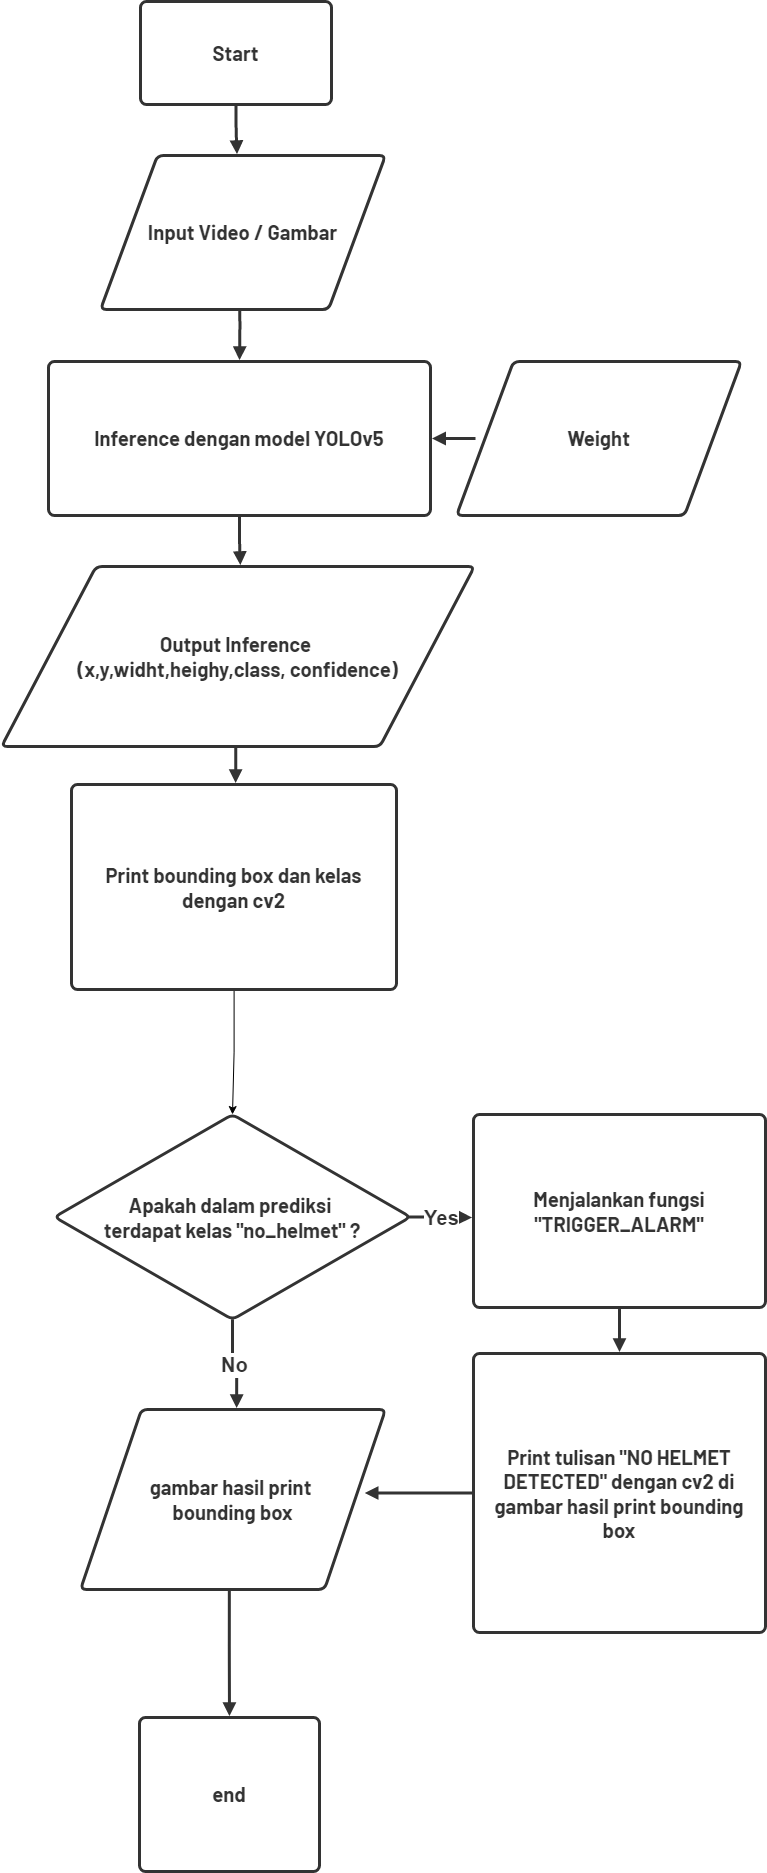
\includegraphics[width=0.4\textwidth]{gambar/utilities/sistemhedect.drawio.png}

  % Ubah sesuai dengan keterangan gambar yang diinginkan.
  \caption{Hardhat Detection System Flowchart}
  \label{fig:flowchart_sistem}
\end{figure}

\begin{figure} [ht]
  \centering
  % Ubah sesuai dengan nama file gambar dan ukuran yang akan digunakan.
  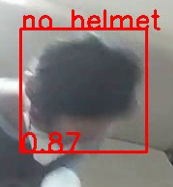
\includegraphics[width=0.2\textwidth]{gambar/utilities/bbox1.png}
  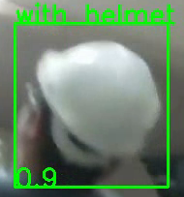
\includegraphics[width=0.2\textwidth]{gambar/utilities/bbox2.png}

  % Ubah sesuai dengan keterangan gambar yang diinginkan.
  \caption{Bounding Box Result}
  \label{fig:bboxresult}
\end{figure}


% \par The alarm function will be executed when one or more 'no\_helmet' 
% class object is detected inside the frame that is being \emph{inferenced} by the model. 
% This alarm function contains commands to play the alarm audio to simulate a siren alarm. 
% In addition to running the alarm function, it will also run a command to display 
% “NO\_HELMET DETECTED” on the predicted frame as shown in Figure~\ref{fig:alarmtriggerexample}.

\par Fungsi alarm akan dijalankan ketika dalam frame yang sedang di-\emph{inference} terdeteks objek dengan \emph{class} bernama \emph{“no\textunderscore helmet”}. Fungsi alarm ini berisi perintah untuk memainkan audio alarm untuk mensimulasikan sirine alarm. Selain menjalankan fungsi alarm, akan juga dijalanan perintah untuk mendisplay text \emph{“NO HELMET DETECTED”} pada frame yang sedang di-\emph{inference} seperti yang ditunjukan pada Gambar~\ref{fig:alarmtriggerexample}.

\begin{figure} [ht]
  \centering
  % Ubah sesuai dengan nama file gambar dan ukuran yang akan digunakan.
  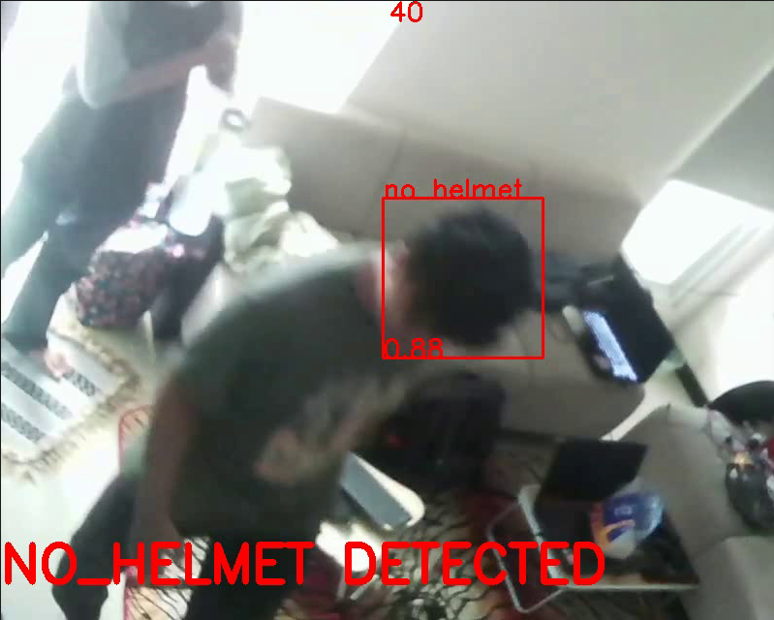
\includegraphics[width=0.4\textwidth]{gambar/utilities/alarm_example.png}

  % Ubah sesuai dengan keterangan gambar yang diinginkan.
  \caption{Contoh Saat Alarm Menyala}
  \label{fig:alarmtriggerexample}
\end{figure}

% \par As an addition, the Frame-rate counter will be shown on the middle top of the window of the output. This is done as a way to benchmark the performance of each model that is being tested in this research where YOLOv5 provides a Small variant to a Large variant. It is expected the larger the model, the smaller the frame per second (FPS) will be.

\par Sebagai tambahan, FPS \emph{counter} akan ditampilkan di tengah atas jendela output. Hal ini dilakukan sebagai cara untuk membandingkan performa dari setiap model yang sedang diuji dalam penelitian ini dimana YOLOv5 menyediakan varian Small hingga varian Large. Diharapkan semakin besar modelnya, semakin kecil frame per second (FPS).